\frame{
  \frametitle{Merkle Tree\footnote{Merkle, R. C. (1979)}}
  \begin{columns}
      \begin{column}{0.4\textwidth}
          \begin{itemize}
            \item Tree of hashes, widely used for data verification
            \begin{itemize}
                \item Cryptographic schemes
                \item P2P file sharing
                \item Distrbuted filesystems
            \end{itemize}
            
            \medskip

            \item Each internal node hashes the concatenated hashes of their children.

            \medskip

            \item Only recomputes $O(\log n)$ hashes when data changes!
          \end{itemize}
      \end{column}
        \begin{column}{0.6\textwidth}
            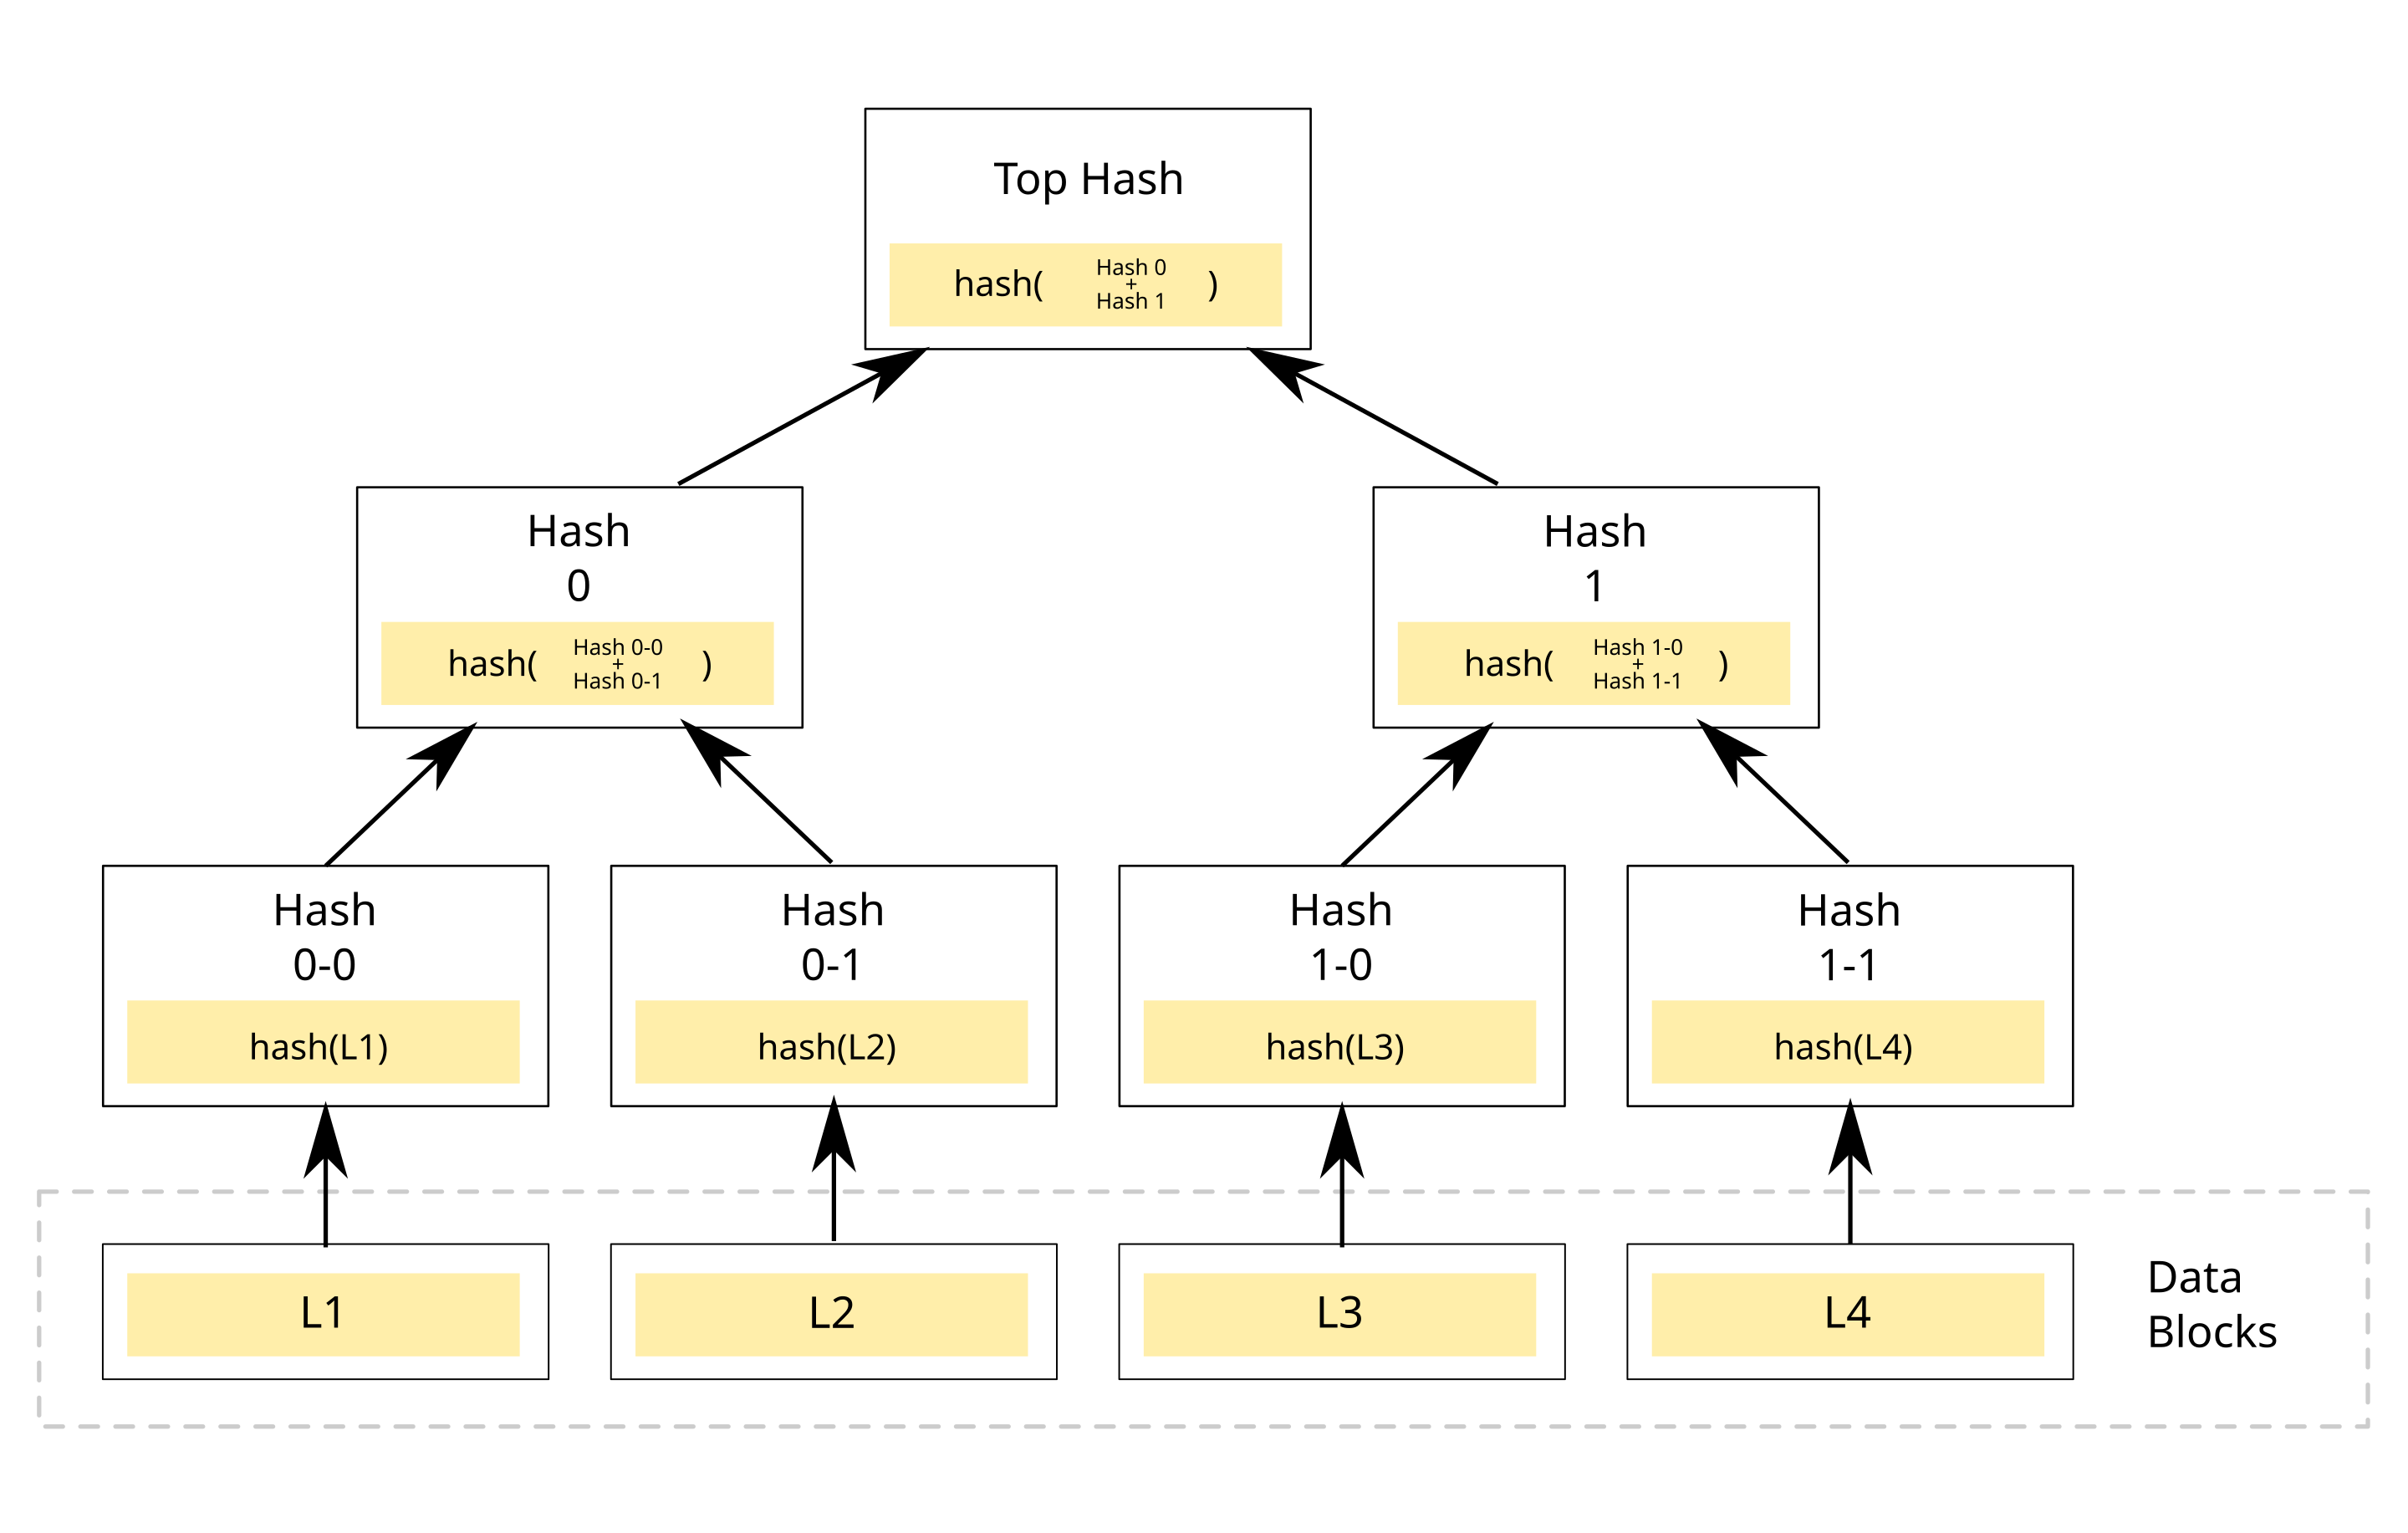
\includegraphics[scale=0.09]{slides/alphabet_trees/merkle_tree.png}
        \end{column}
  \end{columns}
    
}